\chapter{Using Epigrass} 
\label{ch:usingepg}

\lettrine{T}{o} simulate an epidemic process in EpiGrass, the user needs to have in hand three files: Two files containing the site and edge data and a third file which is a script that defines what it is to be done. Here we go through each one of them in detail. As the last part of this chapter, is a step-by step guide the Graphical User Interface (GUI).

\section{Data}

\subsection{Site data file}
See below an example of the content of a site file for a network of 10 cities. Each line corresponds to a site (except the first line which is the title). For each site, it is declared, in this order: its \textit{spatial location} in the form of a pair of coordinates ([X,Y]); a site $name$ to be used in the output; the site's population; the site geocode (an arbitrary unique number which is used internally by EpiGrass).

\begin{lstlisting}[frame=trBL, caption= ,label=]
X,Y,City,Pop,Geocode
1,4,"N1",1000000,1
2,4,"N2",100000,2
3,4,"N3",1000,3
4,4,"N4",1000,4
5,4,"N5",1000,5
1,3,"N6",100000,6
2,3,"N7",1000,7
3,3,"N8",100000,8
4,3,"N9",100000,9
5,3,"N10",1000,10
1,2,"N11",1000,11
\end{lstlisting}

In this example, the first site is located at $[X,Y]=[1,4]$, it is named N1, its population is 1000000 and its geocode is 1. This is minimum configuration of a site data file and it must contains this information in exactly this order. 

In some situations, the user may want to add other attributes to the sites (different transmission parameters, or vaccine coverage or initial conditions for simulations). This information is provided by adding new columns to the minimum file. For example, if one wishes to add information on the vaccine coverage in cities N1 to N10 ($vac$) as well as information about average temperature (which hypothetically affects the transmission of the disease), the file becomes:

\begin{lstlisting}[frame=trBL, caption= ,label=]
X,Y,City,Pop,Geocode,Vac,Temp
1,4,N1,1000000,1,0.9,32
2,4,N2,100000,2,0.88,29
3,4,N3,1000,3,0.7,25
4,4,N4,1000,4,0.2,34
5,4,N5,1000,5,0,26
1,3,N6,100000,6,0,27
2,3,N7,1000,7,0,31
3,3,N8,100000,8,0,30
4,3,N9,100000,9,0,24
5,3,N10,1000,10,0,31
\end{lstlisting}

During the simulation, each site object receives these informations and store them in appropriate variables that can be used later during model specification. Population is stored in the variable $N$; while the extra columns (those beyond the geocode) are stored in a tuple named \textit{values}. For example, for the city $N1$, we have $N = 1000000$ and $values=[0.9,32]$. During model specification, we may use $N$ to indicate the population size and/or we can use $values[0]$ to indicate the level of vaccination of that city and $values[1]$ to indicate the temperature. 

It is up to the user, to know what means the elements of the tuple $values$. Note that the first element of the tuple has index 0,the second one has index 1 and so on.

When using real data, one may wish to use actual geocodes and coordinates. For example, for a network of Brazilian cities, one may build the following file:


\begin{lstlisting}[frame=trBL, caption= ,label=]
latitude,longitude,local,pop,geocode
-16:19:41,-48:57:10,ANAPOLIS,280164,520110805
-10:54:32,-37:04:03,ARACAJU,461534,280030805
-21:12:27,-50:26:24,ARACATUBA,164449,350280405
-18:38:44,-48:11:36,ARAGUARI,92748,310350405
-21:13:17,-43:46:12,BARBACENA,103669,310560805
-22:32:53,-44:10:30,BARRA_MANSA,165134,330040705
-20:33:11,-48:34:11,BARRETOS,98860,350550005
-26:54:55,-49:04:15,BLUMENAU,241943,420240405
-22:57:09,-46:32:30,B.PAULISTA,111091,350760505
\end{lstlisting}



In this file, the coordinates are the actual geographical latitude and longitude coordinates. This information is important when using EpiGrass integrated with Grass GIS. The geocode is also the official geocode of these localities. Despite the cumbersome size of the number, it may be worth using it because demographic official databases are often linked by this number.



\subsection{Edge data file}

The edge data file contains all the direct links between sites. Each line in the file (except the first) corresponds to an edge. For each edge (or link) one must specify (in this order): the \textit{names of the sites} connected by that edge; the \textit{number of individuals traveling from source to destination}; the \textit{number of individuals travelling from destination to source} per time step; the \textit{distance or length} of the edge. At last, the file must contain, in the fifth and sixth columns, the \textit{geocodes of the source and destination sites}. This is very important as graph is built internally connecting sites through edges and this is done based on geocode info. 

\vspace{1cm}
\textbf{IMPORTANT: It is required that the order of columns is kept the same}
\vspace{1cm}

See below the list of the 8 edges connecting the sites $N1$ to $N10$. Let's look the first one, as an example. It links $N1$ to $N2$. Through this link passes 11 individuals backwards and forwards per time step (a day, for example). This edge has length 1 (remember that $N1$ is at [X,Y]=[1,1] and $N2$ is at [X,Y]=[1,2], so the distance between them is 1). The last two columns show the geocode of $N1$ (geocode 1) and the geocode of $N2$ (geocode 2).

\begin{lstlisting}[frame=trBL, caption= ,label=]
Source,Dest,flowSD,flowDS,Distance,geoSource,geoDest
N1,N2,11,11,1,1,2
N2,N4,0.02,0.02,1,3,4
N3,N8,1.01,1.01,1,3,8
N4,N9,1.01,1.01,1,4,9
N5,N10,0.02,0.02,1,5,10
N6,N5,1.01,1.01,1,7,8
N7,N10,1.01,1.01,1,7,8
N9,N10,1.01,1.01,1,9,10
\end{lstlisting}

Note that it doesn't matter which site is considered a Source and which one is considered a Destination. I.e., if there is a link between $A$ and $B$, one may either named $A$ as source and $B$ as destination, or the other way around.

If the edge represents a road or a river, one may use the actual metric distance as length. If the edge links arbitrary localities, one may opt to use euclidean distance, calculated from the x and y coordinates (using Pitagoras theorem). 



\section{Specifying a model: the script}

Once the user has specified the two data files, the next step is to define the model to be executed. This is done in the .EPG script file. The .EPG script is a text file and can be edited with any editor (not word processor). This script must be prepared with care. 

The best way to write down your own .EPG is to edit an already existing .epg file. So, open \textbf{EpiGrass}, choose an .epg file and click on the \textbf{Edit} button. Your favorite editor will open and you can start editing. Don't forget to save it as a new file in your working directory. Of course, there is an infinite number of possibilities regarding the elaboration of the script. It all depends on the goals of the user. 

For the beginner, we suggest him/her to take a look at the .epg files in the demo directory. They are all commented and may help the user in getting used with Epigrass language and capabilities.

Some hints to be successful when editing your .EPG:

\begin{itemize}
\item  All comments in the script are preceeded by the symbol \#. These comments may be edited by the user as he/she wishes and new lines may be added at will. Don't forget, however, to place the symbol \# in every line corresponding to a comment.
\item The script is divided into a few parts. These parts have capital letter titles within brackets. Don't touch them!
\item Don't remove any line that is \textit{not} a comment. See below how to appropriately edit these command lines. 
\end{itemize}

Let's take a look now at each part of a script (this is the script.epg demo file):

\subsection{PART 1: THE WORLD}

The first section of the script is titled: THE WORLD. An example of its content is shown:
 
\begin{lstlisting}[basicstyle=\footnotesize,language=Python, frame=trBL, caption= ,label=]
#=========================================================#
[THE WORLD]
#=========================================================#

location = BRASIL
vector layer = Limite_politico_administrativo
sites = sitios2.csv
edges = edgesout.csv
\end{lstlisting}

where 

\begin{description}
\item[location:] indicates the GRASS location where maps (raster and vector maps) for the region are stored (required only if GRASS location exists. If not, leave it blank: $location =$ ). 
\item[vector layer:] Name of the vector layer, in the GRASS location, to be used as background to the network visualizer. 
\item[sites:] this is the name of the .CSV file containing the list of sites and their attributes.
\item[edges:] this is the name of the .CSV file containing the list of edges and their attributes.
\end{description}

\subsection{PART 2: EPIDEMIOLOGICAL MODEL}

This is the main part of the script. It defines the epidemiological model to be run.
The script reads:

\begin{lstlisting}[basicstyle=\footnotesize,language=Python, frame=trBL, caption= ,label=]
#=========================================================#
[EPIDEMIOLOGICAL MODEL]
#=========================================================#
#model types available: SIS, SIS_s ,SIR, SIR_s, SEIS, SEIS_s, SEIR, SEIR_s, 
# SIpRpS, SIpRpS_s,SIpR,SIpR_s(see documentation for description)
modtype = SIR

\end{lstlisting}

Here, the type of epidemiological model is defined, in this case is a deterministic SIR model. EpiGrass has some built-in models:


\begin{center}
\begin{tabular}{l l l}
\hline 
\textbf{Model}	&\textbf{Detemrinistic} &\textbf{Deterministic}. \\ \hline	
Susceptible-Infected-Recovered  & $SIR$	& $SIR_s$\\
Susceptible-Exposed-Infected-Recovered & $SEIR$	& $SEIR_s$\\
Susceptible-Infected-Susceptible & $SIS$  &  $SIS_s$\\
Susceptible-Exposed-Infected-Susceptible & $SEIS$ & $SEIS_s$\\
SIR with fraction with full immunity & $SIpRpS$ & $SIpRpS_s$\\
SEIR with fraction with full immunity & $SEIpRpS$ & $SEIpRpS_s$\\
SIR with partial immunity for all & $SIpR$ & $SIpR_s$\\
SEIR with partial immunity for all & $SEIpR$ & $SEIpR_s$\\
SIR with immunity wane & $SIRS$ & $SIRS_s$\\
\hline
\end{tabular}
\end{center}

A description of these models can be found in section \ref{cap:modeling}. The stochastic models use Poisson distribution as default for the the number of new cases ($L_{t+1}$). Following the script, we find:

\begin{lstlisting}[basicstyle=\footnotesize,language=Python, frame=trBL, caption= Defining model parameter and initial values ,label=lst:pars]
#==============================================================#
[MODEL PARAMETERS]
#==============================================================#

#  They can be specified as constants or as functions of global or 
#  site-specific variables. these site-specific variables, are provided
#  in the sites file. All the numbers given after the geocode (4th column)
#  are collected into the values tuple.
# Examples:
# beta = 0.001
# beta=values[0] #assigns the first element of values to beta 
# beta=0.001*values[1]

beta = 0.4   #transmission coefficient (contact rate * transmissibility)
alpha = 1  # clumping parameter
e = 1   # inverse of incubation period
r = 0.1   # inverse of infectious period
delta = 1  # probability of acquiring full immunity [0,1]
B = 0           # Birth rate
w = 0           # probability of immunity waning [0,1]
p = 0           # 

\end{lstlisting}

These are the model parameters, as described in \ref{Table:symbols}. Not all parameters are necessary for all models. For example, $e$ is only required for SEIR-like models. Don't
remove the line, however because that will cause an error. We recommend that, if the parameter is not necessary, just add a comment after it as a reminder that it is not being used by the model.

In some cases, one may wish to assign site-specific parameters. For example, transmission rate may be different between localities that are very distant and are exposed to different climate. In this case site specific variables can be added as new columns to the site file. All columns after the geocode are packed into a tuple named \textit{values} and can be referenced as shown in listing \ref{lst:pars}. I.e., the first element of the tuple is values[0], the second element is values[1], the third element is values[2] and so on.

The next part of the script, the initial conditions are defined. Here, the number of individuals in each epidemiological state, at the start of the simulation, is specified.The script reads:

\begin{lstlisting}[basicstyle=\footnotesize,language=Python, frame=trBL, caption= ,label=]
[INITIAL CONDITIONS]

# Here, the number of individuals in each epidemiological
# state (SEI) is specified. They can be specified in absolute
# or relative numbers.
# N is the population size of each site.
# The rule defined here will be applied equally to all sites.
# For site-specific definitions, use EVENTS (below)
# Examples:
#	S,E,I = 0.8*N, 10, 0.5*N
#	S,E,I = 0.5*N, 0.01*N, 0.05*N
#	S,E,I = N-1, 1, 0
S = N
E = 0
I = 0
\end{lstlisting}

Here, $N$ is the total population in a site (as in the datafile for sites). In this example, we set all localities to the same initial conditions (all individuals susceptible) and use an event (see below) to introduce an infectious individual in a locality. The number of recovered individuals is implicit, as $R = N-(S+E+I)$

Another possibility is to define initial conditions that are different for each site. For this, the data must be available as extra columns in the site datafile and these columns are referrenced to using the \textit{values} tuple explained above.

The next step is to define events that will occur during the simulation. These events may be epidemiological (arrival of an infected, for example) or a public health action (vaccination campaign, for example):

\begin{lstlisting}[basicstyle=\footnotesize,language=Python, frame=trBL, caption=Defining epidemic events ,label=lst:event]
[EPIDEMIC EVENTS]

# Specify isolated events.
# Localities where the events are to take place should be Identified by a numeric code 
# to come after population size on the sites data file.
# Seed : [('locality1's geocode', n),('locality2's geocode', n)]. 
# N infected cases will be added to locality at time 0.
# Vaccinate: [('locality1's geocode', time, coverage),('locality2's geocode', time, coverage)] 
# Quarantine: [(locality1's geocode,time,duration), (locality2's geocode,time,duration)]
seed = [(230440005,1)] #Fortaleza
Vaccinate = [(355030800, 31, 0.9)] #Sao Paulo
Quarantine = [(355030800,20)]
\end{lstlisting}

The events currently implemented are:
\begin{description}
\item{seed} One infected individual is introduced into a site. The notation for a single event is:
$$seed = [(geocode,time step)]$$
For example, $seed = [(2,1)]$ programs the arrival of an infected individual at site geocode 2, at time 1. 
For several events, the notation is:
$$seed = [(geocode1,time step1),(geocode2,time step2),(geocode3,time step3)]$$
There is no limit to the number of events that can be included in this list.
\item{Vaccinate} Implements a campaign that vaccinates a fraction of the population in a site, at a pre-defined time-step. For a single event, the notation is:
$$[(geocode1, time, coverage)]$$
where the first element is the geocode of the city, the second element is the time when the campaign is implemented and the third element is the coverage. For example, the event $[(2,10,0.7)]$ means that city 2, at time 10, has 70\% of its population vaccinated. Mathematically, it means (in the model), the removal of individuals from the susceptible to the recovered stage.
For several events, we may have simultaneous vaccinations at two sites:
$$Vaccinate = [(1, 31, 0.9),(2,31,0.9)]$$ 
or subsequent campaigns in the same site:
$$Vaccinate = [(1, 31, 0.2),(1,61,0.3)]$$ 
\item{Quarantine} Prevents any individual from leaving a site, starting at $t$. The notation is:
$$Quarantine = [(geocode1,t),(geocode2,t)]$$
As an example, a quarantine in locality 2, that starts at day 10 is noted:
$Quarantine = [(2,10)]$
\end{description}

\subsection{PART 3: TRANSPORTATION MODEL}

Here, there are two options regarding the movement of infected individuals from site to site (through the edges). If $stochastic = 0$, the process is simulated deterministically. The number of infected passengers commuting through an edge is a fraction $p$ of the infected population that is traveling. $p$ is calculated as $\frac{total passengers}{total population}$ . 

If $stochastic = 1$, the number of passengers is sampled from a Poisson distribution with parameter given by the expected number of travelling infectives (calculated as above).  

\begin{lstlisting}[basicstyle=\footnotesize,language=Python, frame=trBL, caption= ,label=]
#=========================================================#
[TRANSPORTATION MODEL]
#=========================================================#
# If doTransp = 1 the transportation dynamics will be 
# included. Use 0 here only for debugging purposes.
doTransp = 1

# Mechanism can be stochatic (1) or deterministic(0). 
stochastic = 1

\end{lstlisting}

That ends the definition of the model. 
\subsection{SIMULATION AND OUTPUT}
Now it is time to define some final operational variables for the simulation:

\begin{lstlisting}[basicstyle=\footnotesize,language=Python, frame=trBL, caption= ,label=]
#=========================================================#
[SIMULATION AND OUTPUT]
#=========================================================#

# Number of steps
steps = 200

# Output dir
outdir = ~/data

# Output file
outfile = simul.dat

# Database Output
# MySQLout can be 0 (no database output) or 1
MySQLout = 1 

# Graphical outputs
draw map = 1

# Report Generation
# The variable report can take the following values:
# 0 - No report is generated.
# 1 - A network analysis report is generated in PDF Format.
# 2 - An epidemiological report is generated in PDF Format.
# 3 - A full report is generated in PDF Format.
# siteRep is a list with site geocodes. For each site in this list, a detailed report is apended to the main report.
report = 0
siteRep = [230440005,355030800]

#Batch Run
#  list other scripts to be run in after this one. don't forget the extension .epg
#  model scripts must be in the same directory as this file or provide full path.
#  Example: Batch = ['model2.epg','model3.epg','/home/jose/model4.epg']
Batch = []
\end{lstlisting}

where
\begin{description}
\item[step] Number of time steps for the simulation.
\item[outdir] Directory for data output (currently not in use)
\item[outfile] .csv filename that can be imported into R as a dataframe. This .csv file contains the simulated timeseries for all nodes.
\item[MySQLout] Use MySQLout $= 1$ if simulated time series are to be stored in MySQL database. Time series of $L$,$S$,$E$,and $I$, from simulations, are stored in a MySQL database named \emph{epigrass}. The results of each individual simulation is stored in a different table named after the model's script name, the date and time the simulation has been run. For instance, suppose you run a simulation of a model stored in a file named \texttt{script.epg}, then at the end of the simulation, a new table in the epigrass database will be created with the following name: \texttt{script\_Wed\_Jan\_26\_154411\_2005}. Thus, the results of multiple runs from the same model get stored independently.
\item[draw map]
\item[report]Three types of report are currently available: $Report = 1$ returns a set of descriptors of the network, described in \ref{cap:analysis}; $Report = 2$ returns a set of basic epidemiological measures and plots of the time series; $Report = 3$ is $Report 1 + Report 2$. Report Generation is an optional, though recommended, step done at the end of the simulation. For the report, descriptive statistics are generated for the network. These have to do with network topology and properties. Additional sections can be added to the report with basic statistical analyses of the output of pre-selected nodes, listed  in the $siteRep$ variable at the script.
\item[siteRep=[]] List of nodes for which network and epidemiological measures are to be calculated and included in the report.
\item[Batch=[]] script files included in this list are executed after the currently file is finished.
\end{description}
\section{User defined models}
In future releases Epigrass will allow the user to define epidemiological models to be included into the sites.


\section{Using Epigrass for specific tasks}

Here we describe some things you could do with epigrass and some specific hints:

\subsection{Describing a network}
A user wants to obtain the topological properties of a network. Reasons for this could be: 1) learn how to interpret these measures, 2) describe a air transportation or a road transportation network. To do that, you need:

\begin{description}
\item[Set steps = 1]. If no model of disease is needed, then most of the .epg script can be ignored. Don't remove anything, however, from the script.  Note that Epigrass requires a model in order to work properly, even if the user does not want it. One solution to reduce the run time, in this case, is to set \textbf{steps} to 1 (steps = number of steps in the simulation).
\item[Set MySQLout = 0]. Network measures are not sent to database.
\item[Set report = 1]. Report 1 calculates network measures and save them in a .pdf file.
\item[Especify siteRep]. If siteRep = [], only global network measures are included in the report. If site-specific measures are needed, include their geocodes in the list siteRep. For example, to calculate site stats for all nodes, mesh1.epg has:
\begin{verbatim}
report = 1
siteRep = [1,2,3,4,5,6,7,8,9,10,11,12,13,14,15,16,17,18,19,20]
\end{verbatim}
\end{description}

Script mesh1.epg is configured this way. Run it and take a look at the report. 


\subsection{Comparing networks}
A user wants to compare the properties of a set of networks. Reasons for this could be: 1) learn how to interpret these measures, 2) describe/compare a air transportation to a road transportation network, 3) analyse how network topology changes by adding/removing specific nodes or edges.

If there are four graphs, then four .epg files must be created. They all must set $report=1$ and $siteRep$ to the desired specification (as above). Each file must be executed and each one will provide a report. 

To quick thinks a little bit, the script allows the user to choose one of the files as a master file. In the option $BatchRun$, one may list the other scripts to be run after this one. They all must be in the same directory as the master file (or you may provide full path).

For example, suppose you want to compare the topologies of the four networks displayed in \ref{fig:artgraphs}.
 
 \begin{center}
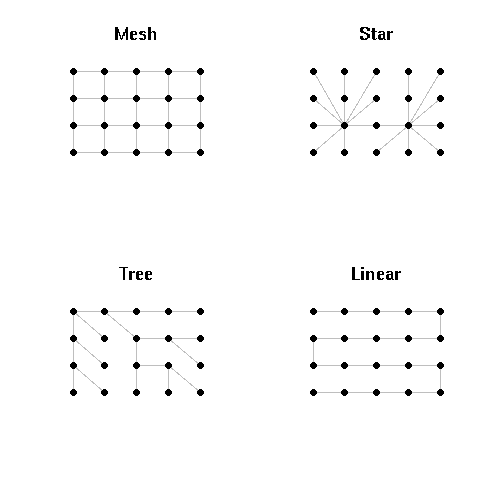
\includegraphics[scale=0.5]{artgraphs.png}
%\caption{SIR-like models}
\label{fig:artgraphs}
\end{center}

 
We created four files (mesh2.epg, star2.epg, lin2.epg, tree2.epg) and used one of them as master (mesh2.epg). The four files are exactly the same, except for the name of the edge file and the \textbf{Batch} specification. I.e., in mesh2.epg we specify:
\begin{verbatim}
Batch = ['star2.epg','lin2.epg','tree2.epg']
\end{verbatim}
Now, mesh2.epg is run. One report will be delivered for each script (In future version of Epigrass, a more integrated result is planned). From the reports, we get network measures for the four graphs. These network measures are explained in chapter \ref{cap:analysis}). 


\subsection{Simulate disease spread from a single site}
The user specifies a network (let's say, a tree network) and wishes to simulate disease spread in this network. The graph is disease-free at time 0. At time 1, an infected person arrives at site $N1$. No control measures are introduced. The model chosen is SipRpS. 
The script file tree3.epg was built following these guidelines:
\begin{description}
\item[Initial conditions] All individuals are initially susceptible, i.e.,  $S=N$.  
\item[Epidemic events] An infected individual arrives at time 1 in N1.
\item[steps=200] This may be increased or reduced, depending on the parameters.
\item[Report = 2]. Report 2 returns only the epidemiological results.
\item[Specify siteRep]. If site-specific measures are needed, include their geocodes in the list siteRep. For example, to calculate site stats for three nodes, tree3.epg has:
\begin{verbatim}
report = 2
siteRep = [1,12,14]
\end{verbatim}
Run this script and take a look at the report. A sugestion: change the script and seed the disease in a more central node. See how this affect the velocity of disease propagation.
\end{description}

\subsection{Simulating vaccination campaigns}
Vaccination may be simulated in different ways, using the section Epidemic Events in the script. These are some examples:
\begin{description}
\item[A single, local campaign].  In site N1, exactly at time 10, with coverage 0.5
\begin{verbatim}
Vaccinate = [(1,10,0.5)]
\end{verbatim}
\item[Simultaneous campaigns in three sites].  In sites N1, N4 and N6, exactly at time 10, with coverage 0.5
\begin{verbatim}
Vaccinate = [(1,10,0.5),(4,10,0.5),(6,10,0.5)]
\end{verbatim}
\item[Campaign with a time span].  In site N1, a campaign that occurs from day 10 to day 15, with daily coverage of 0.1.
\begin{verbatim}
Vaccinate = [(1,10,0.1),(1,11,0.1),(1,12,0.1),(1,13,0.1),
(1,14,0.1),(1,15,0.1)]
\end{verbatim}
\end{description}


\subsection{Simulating quarantines}
Quarantines are simulated similarly to vaccinations, but once they are initiated, they last until the end of the simulation:
\begin{description}
\item[Quarantine in a single place].  In site N1, starting at time 10, with coverage 0.2
\begin{verbatim}
Quarantine = [(1,10,0.2)]
\end{verbatim}
\item[Quarantine in two places].  In sites N1 and N3, at times 10 and 12, respectively, with coverage 0.5
\begin{verbatim}
Quarantine = [(1,10,0.5),(3,12,0.5)]
\end{verbatim}
\item[Quarantine with a time span].  In site N1, a quarantine that starts at day 10 and ends at time 30, with daily coverage of 0.75.
\begin{verbatim}
Quarantine = [(1,10,0.75),(1,30,0)]
\end{verbatim}
\end{description}

\subsection{Comparing strategies}
One goal of modeling diseases is to compare alternative control measures in terms of number of cases prevented. A set of scripts may be prepared to compare six alternative strategies for controlling the spread of an epidemic in the star graph, that was initiated at time 4 in site N1. For example:
\begin{description}
\item[Strategy vac1]  Vaccinate site $N1$, at time $7$, with coverage $0.8$ .
\item[Strategy vac2]  Vaccinate sites $N1$, $N12$ and $N14$, at time $7$, with coverage $0.8$. $N12$ and $N14$ are central nodes of the star network and are natural candidates for vaccination.
\item[Strategy mixed] Strategy vac1 $+$ quarantine in sites $N12$ and $N14$, coverage of $0.7$.
\item[Strategy quar] Quarantine in sites $N1$, $N12$ and $N14$, coverage of $0.7$.
\end{description}


\section{The Graphical User Interface(GUI)}
Epigrass comes with a simple but effective GUI(figure \ref{fig:gui}), that allows the user to control some aspects of the run-time behavior of the system. The Gui can be invoked by typing \texttt{epigrass} in prompt of a console. We suggest the user to start EpiGrass from the same directory where his/her model definition is located (.csv and .epg files).

All the information that is entered via the GUI gets  stored in a hidden file called \texttt{.epigrassrc} stored in the home folder of the user. Every time the GUI is invoked, the data stored in the \texttt{.epigrassrc} file is used to fill the forms in the GUI. The gui is designed as a tabbed notebook with four tabs (Run Options, Settings, Utilities, and Visualization).

At the bottom of the Gui there are three buttons \texttt{Help}, \texttt{Start} and \texttt{Exit}. Their functions will be explained below. Immediately above the \texttt{Run} and \texttt{Exit} buttons, there is a small numeric display that will display the simulation progress after it has been started.
\begin{figure}
	\centering
%	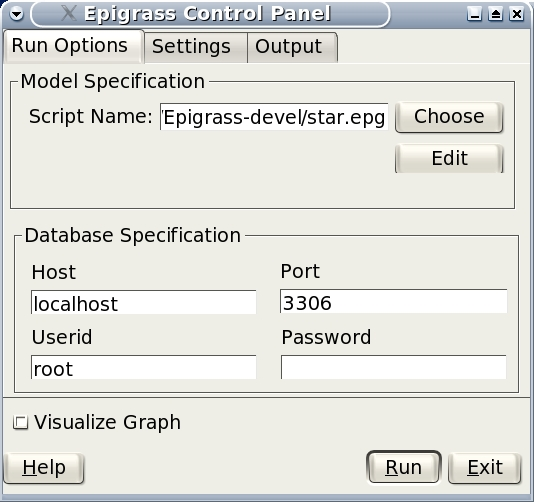
\includegraphics[scale=0.7]{gui.jpg}
% gui.jpg: 72dpi, width=18.84cm, height=17.71cm, bb=0 0 534 502
	\caption{First tab of the EpiGrass GUI.}
	\label{fig:gui}
\end{figure}

\subsection{Run Options}
The first tab of the GUI(figure \ref{fig:gui}), contains a number of variables that, with the exception of the model script filename, should remain the same for most simulations you are going to run.

On the top of the first tab is a text box to enter the file name of the model script (\texttt{something.epg}). By clicking on the \texttt{Choose} button at the right of this box, you get a file selection dialog to select your script file. If you need you can click on the \texttt{Edit} button below to edit the script file with your favorite text editor.

Below, you can enter details about the MySQL database that will store the output of your simulations. Here you can enter the server IP, port, user and password. On the first time you run the GUI these input boxes will be filled with the default values for these variables (server on localhost, port 3306, user epigrass and password epigrass)

\subsection{Settings}
On the settings page, you can enter personal details such as user name (To be used in the simulation report), preferred text editor and preferred PDF reader. The preferred text editor will be used to open your script from the GUI, when you click on the edit button in the first tab. The PDF reader specified, will be used to open the report file, when requested (Utilities tab) and the user manual, when the user clicks on the help button on the bottom-left corner of the GUI.

On this tab, the language of the GUI can also be selected from a list of available translations. The effects of language changes will only take place when the next time the GUI is started.
\begin{figure}
	\centering
%	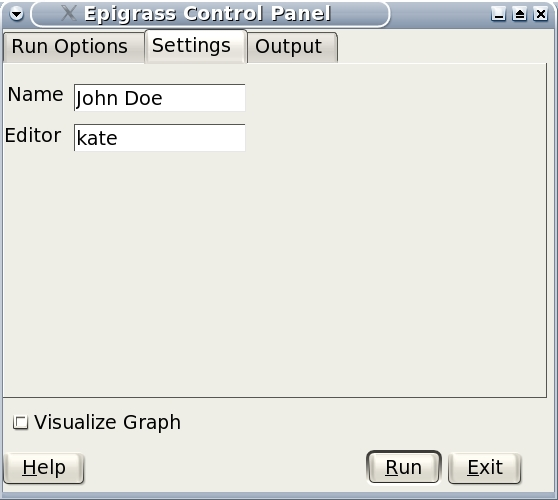
\includegraphics[scale=0.7]{guiset.jpg}
% guiset.jpg: 72dpi, width=19.68cm, height=17.64cm, bb=0 0 558 500
	\caption{Second tab of the GUI.}
	\label{fig:guiset}
\end{figure}

\subsection{Utilities}
In the Utilities tab, you can get feed back from the simulator. Especially during long simulation runs, it is good to know how it is progressing. During the simulation, text messages regarding the status of the simulation are written to the text box on the left. 
\begin{figure}
	\centering
%	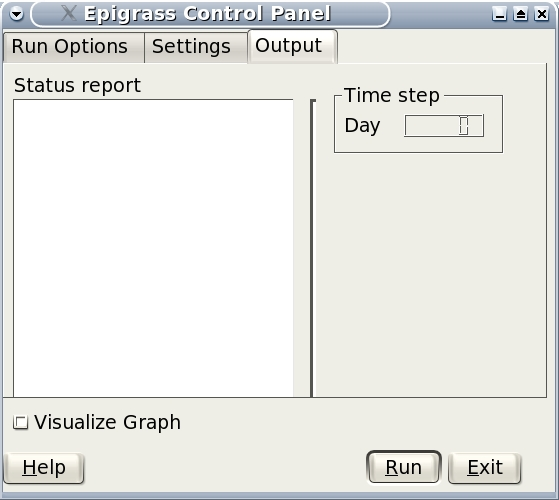
\includegraphics[scale=0.7]{guiout.jpg}
% guiout.jpg: 72dpi, width=19.72cm, height=17.64cm, bb=0 0 559 500
	\caption{Third tab of the GUI}
	\label{fig:guiout}
\end{figure}

On the right, there is a button for backing up the data base and another for opening the report generated by the last simulation. Since report PDFs ar stored in folder directly below the ones on which the simulation is started, older reports should still be accessible and can be opened directly by selecting the desired report using the operating system's file manager.

\subsection{Visualization}
The fourth tab of the GUI is the visualization Tab. This tab was designed for playing animations of any simulation data that is stored in the database. Pressin the \texttt{Scan DB} button, causes the available tables in the  epigrass database to be listed in the \texttt{Simulations stored} combo box. The user can then select one of these simulations to visualize.

Once the \texttt{Start animation} button is pressed, a graphical display window pops up, and the simulation is replayed at a speed given by the frame rate set by the user  or the maximum speed of the computer (whichever is smaller). In the animation, the nodes of the network are represented by boxes whose volume is given by the number of infected at each node. The node colors are as following: Green for uninfected nodes, and red to blue for infected nodes. bright red for for first infected node with the nodes becoming infected later assuming a color with progressively more blue.


Maps can also be selected from the \texttt{Maps availabled combo box} to be used as background for the network display. The maps must be in the GRASS ascii vectorial format and have coordinates compatible with those given to the nodes of the simulation.

\subsection{Operation}
After all the information has been entered and checked on the GUI, you can press the \texttt{Run} button to start the simulation or the \texttt{Exit} button. When the \texttt{Run} button is pressed, the \texttt{.epigrassrc} file is updated with all the information entered in the gui. If the \texttt{Exit} button is pressed, all information entered since the last time the \texttt{Run} button was pressed is lost.

